\subsubsection{Propriedades da Função Tangente}

\begin{proposition}
    Valem as seguintes propriedades acerca da função tangente:

\begin{enumerate}[(a)]
  \item Embora não seja definida para todo número real, a função
  tangente pode ser considerada uma função periódica de período
  $\pi$ em todo o seu domínio, pois $\tan \paren{x+\pi} = \tan x$;
  \item Para todo par de pontos  $(x_1, y_1)$ e $(x_2, y_2)$ em uma reta não vertical, com $x_1 \neq x_2$, se
  $\alpha$ é o ângulo formado pela reta e o eixo $x$, então $$\tan
  \alpha = \frac {y_2 - y_1} {x_2 - x_1}.$$
  \item Ao definirmos $tan: \paren{- \frac {\pi} 2, \frac {\pi} 2} \to \reais$,
obtemos uma bijeção. Assim, o intervalo aberto $\paren{- \frac {\pi}
2, \frac {\pi} 2}$ tem a mesma cardinalidade que $\reais$.
\end{enumerate}
\end{proposition}

\begin{proof}
  \begin{enumerate}[(a)]
    \item[]
    \item Seja $x \in \bigcup_{k \in \Z} \paren{k \pi - \frac{\pi} 2, k \pi + \frac {\pi} 2}$. 
  Segue que: $$\tan \paren{x+\pi} = \frac{\sen \paren{x+\pi}}{\cos \paren{x+\pi}}= \frac{-\sen x}{-\cos x}= \frac{\sen x}{\cos x}= \tan x.$$
  Logo, pela Definição~\ref{def:funcao-periodica}, a função tangente é periódica.
  \item Considere uma reta não vertical com equação $y=mx+n$, em que $m > 0$. 
  Considere, também, que essa reta forma um ângulo $\alpha$ com o eixo $x$. 
  Agora, sejam $\paren {x_1, y_1}$ e $\paren{x_2, y_2}$ pontos quaisquer da reta tais que $x_1 \neq x_2$. 
  O esquema é ilustrado na Imagem~\ref{img:prova-props-tangente}. 
  %
  \begin{figure}[H]
      \centering
      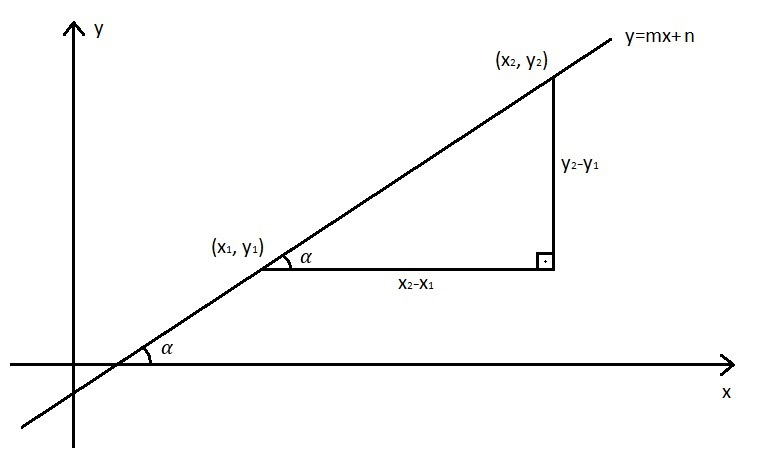
\includegraphics[scale=0.65]{\imgdirfromsection/props-tangente.jpg}
      \caption{Reta $y = mx + n$ e os pontos $\prn{x_1, y_1}$ e $\prn{x_2, y_2}$.}
      \label{img:prova-props-tangente}
  \end{figure}
    %
  No triângulo retângulo formado na imagem, temos:
  \begin{align*}
    \tan \alpha &= \frac {\sen\alpha}{\cos\alpha} \\ 
    &= \frac{ \frac{\text{cateto oposto}}{\text{hipotenusa}}   }{\frac{\text{cateto adjacente}}{\text{hipotenusa}}} \\
    &= \frac{\text{cateto oposto}}{\text{cateto adjacente}}\\
    &= \frac{y_2 - y_1}{x_2 - x_1}
  \end{align*}
  %
  O caso em que $m < 0$ é análogo.

  Sabemos que $\frac{y_2 - y_1}{x_2 - x_1} = m$ (Exercício \ref{exer:determinicidade-funcao-afim}).
  É por conta dessa igualdade que o valor $m$ numa função afim é, costumeiramente, chamado de coeficiente angular. Porém, reforçamos que o termo mais apropriado para designar o $m$ numa função afim é taxa de variação ou taxa de crescimento. Use o termo coeficiente angular quando estiver se referindo explicitamente a uma reta. Nesse contexto, ele corresponde ao valor da tangente de $\alpha$, o ângulo formado pela reta e o eixo $x$.
  \item A demonstração deste item está fora do escopo do texto.
  \end{enumerate}

  
\end{proof}